% Copyright (C) 2007 Technical University of Liberec.  All rights reserved.
%
% Please make a following refer to Flow123d on your project site if you use the program for any purpose,
% especially for academic research:
% Flow123d, Research Centre: Advanced Remedial Technologies, Technical University of Liberec, Czech Republic
%
% This program is free software; you can redistribute it and/or modify it under the terms
% of the GNU General Public License version 3 as published by the Free Software Foundation.
%
% This program is distributed in the hope that it will be useful, but WITHOUT ANY WARRANTY;
% without even the implied warranty of MERCHANTABILITY or FITNESS FOR A PARTICULAR PURPOSE.
% See the GNU General Public License for more details.
%
% You should have received a copy of the GNU General Public License along with this program; if not,
% write to the Free Software Foundation, Inc., 59 Temple Place - Suite 330, Boston, MA 021110-1307, USA.

\normalsize

\subsection{Linear Reactions}
\label{sec:linear_reactions}
The software suppports linear chemical reactions in the transport operator splitting method. 
The linear chemical reactions (we will recall them only as 'reactions' in this section) can desribe
\begin{itemize}
  \item first order kinetic chemical reactions
  \item radioactive decays, their chains and also complex chains with branches.
\end{itemize}
In the first case, the kinetics of a reaction is determined by a kinetic constant \hyperA{Substep::kinetic}{$k$}. 
In the second case, the radioactive decay is determined by the half life of the reactant 
\hyperA{Substep::half-life}{$t_{1/2}$}. Both notations
%
\[ A\xrightarrow{k} B, \qquad A\xrightarrow{t_{1/2}} B \]
%
express the same reaction and are governed by the same first order differential equation 
%
\[ \frac{\d c_A}{\d\tau} = -kc_A = - \frac{\ln 2}{t_{1/2}}\, c_A. \]
%
The relation between $k$ and $t_{1/2}$ is derived below
\begin{eqnarray*}
    \frac{\d c_A}{\d\tau} &=& -k c_A\\
    \frac{\d c_A}{c_A} &=& -k \d\tau\\
    \int\limits_{c_A^0}^{c_A^0/2}\frac{\d c_A}{c_A} &=& -k\int\limits_{0}^{t_{1/2}} 1\d\tau\\
    \big[ \ln c_A\big]^{c_A^0/2}_{c_A^0} &=& -\big[k\tau\big]^{t_{1/2}}_{0}\\
    \ln\frac{c_A^0}{2} - \ln c_A^0 &=& - k t_{1/2}\\
    \ln 2 &=& k t_{1/2}\\
    k &=& \frac{\ln 2}{t_{1/2}}.
\end{eqnarray*}



Lets consider to have a narrow decay chain without branches. This kind of decay chain can be described by following equation
\[
 A\xrightarrow{t_{1/2,A}}B\xrightarrow{t_{1/2,B}}C\xrightarrow{t_{1/2,C}}D\xrightarrow{t_{1/2,D}}E,
\]
where letters $\{A,\ldots, E\}$ denotes isotopes contained in considered decay chain and ${t_{1/2},i},~i\in\{A,\ldots, E\}$ is a symbol for a half-life of $i$-th isotope.
For a simulation of radioactive decay and first order reactions matrix multiplication based approach has been developed. It has been based on an arrangement of all the data to matrices. The matrix ${\bf C}^k$ contains the information about concentrations of all species ($s$) in all observed elements ($e$). The upper index $k$ denotes $k$-th time step. The matrix ${\bf C}^k$ has the dimension $e\times s~( rows \times columns)$.
The transport simulation is realized by matrix multiplication 
\[
  {\bf T}\cdot{\bf C}^k = {\bf C}^{k+1},
\]
where ${\bf T}$ is a square, block-diagonal matrix, representing a set of algebraic equations constructed from a set of partial differential equations.
When the simulation of the radioactive decay or the first order reaction is switched on, one step of
simulation changes to 
\[
  {\bf T}\cdot{\bf C}^k\cdot{\bf R} = {\bf C}^{k+1},
\]
where ${\bf R}$ is a square matrix with the dimension $(s \times s)$ . It is much easier to construct and to use ${\bf R}$ , than to include chemical influence to the transport
matrix ${\bf T}$ , because the matrix ${\bf R}$ has usually a simple structure and $s$ is much smaller than $e$. In the most simple case, when the order of identification numbers of isotopes in considered decay chain is the same as the order of identifiers of species transported by groundwater, then just two
diagonals are engaged and the matrix R looks as follows:

\begin{tiny}\[
   \begin{array}{l}
    {\bf R} = \left(
    \begin{array}{cccccc}
     \left(\frac{1}{2}\right)^\frac{\Delta t}{t_{1/2,1}} & 1 - \left(\frac{1}{2}\right)^\frac{\Delta t}{t_{1/2,i}} & 0 & \hdots & \hdots & 0\\
     0 & \left(\frac{1}{2}\right)^\frac{\Delta t}{t_{1/2,2}} & 1 - \left(\frac{1}{2}\right)^\frac{\Delta t}{t_{1/2,2}} & 0 & \ddots & 0 \\
     \vdots & \ddots & \ddots & \ddots & \ddots & \vdots\\
     0 & \ddots & 0 & \left(\frac{1}{2}\right)^\frac{\Delta t}{t_{1/2,n-2}} & 1 - \left(\frac{1}{2}\right)^\frac{\Delta t}{t_{1/2,n-2}} & 0 \\
     0 & \hdots & \hdots & 0 & \left(\frac{1}{2}\right)^\frac{\Delta t}{t_{1/2,n-1}} & 1 - \left(\frac{1}{2}\right)^\frac{\Delta t}{t_{1/2,n-1}}\\
     0 & \hdots & \hdots & 0 & 0 & 1
    \end{array}\right)
   \end{array}
\]\end{tiny}

Every single $j$-th column, except the first one, includes the contribution $1 - \left(\frac{1}{2}\right)^\frac{\Delta t}{t_{1/2,j}},~j\in\{A,\ldots, E\}$ from $(j-1)$-th
isotope with its half-life $t_{1/2,j-1}$. The term $\left(\frac{1}{2}\right)^\frac{\Delta t}{t_{1/2,j}}$ describes concentration decrease caused by the radioactive decay of $j$-th isotope itself. In general cases the matrix ${\bf R}$ can have much more complicated structure, especially when the considered decay chain has more branches.
The implementation of the radioactive decay in Flow123D does not firmly include standard natural decay chain. Instead of that it is possible for a user to define his/her decay chain.

It is also possible to simulate decay chains with branches as picture \ref{pic:dec_branches} shows.

\begin{figure}[htb]
 \centering
 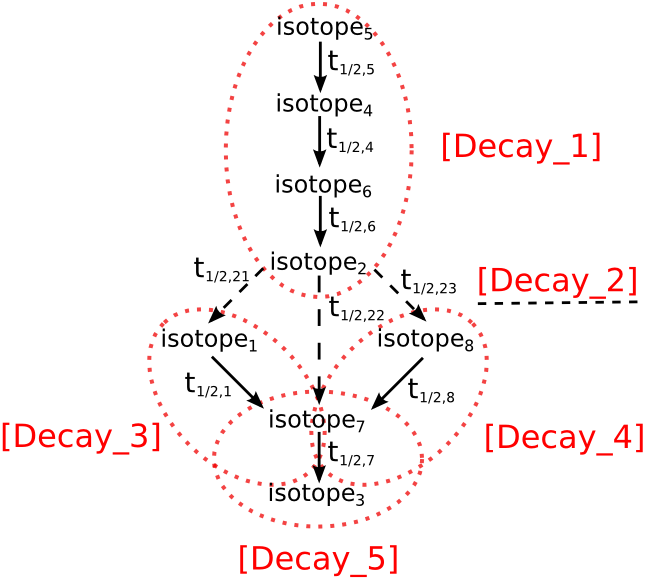
\includegraphics[width = 8cm]{\fig /decay_chain.png}
 \caption{Decay chain with branches.}
 \label{pic:dec_branches}
\end{figure}


When it comes to a simulation of first order reactions, the kinetic constant is given as an input. 
The description of a kinetic chemical reaction has obviously two folowing forms
\[
  \begin{array}{l}
    A\xrightarrow{k}B,\\
    \frac{dc^A}{dt} = -k \cdot c^A.
  \end{array}
\]
The first one description is a standard chemical one. The second equation describes temporal decrease in amount of concentrations of the specie $c^A$. The constant $k$ is so called kinetic constant and for the case of a first order reactions it is equal to so called reaction rate. The order of reaction with just one reactant is equal to the power of $c^A$ in partial diferential reaction.

For an inclusion of first order reaction into a reaction matrix a half-life needs to be computed from the corresponding kinetic constant $k$. The derivation follows
\[
  \begin{array}{l}
    A\xrightarrow{k} B\\
    \frac{dc^A}{d\tau} = -k\cdot c_A\\
    \frac{dc^A}{c^A} = -k\cdot d\tau\\
    \int\limits_{c^A_0/2}^{c^A_0}\frac{dc^A}{c^A} = -k\cdot\int\limits_{t_{1/2,A}}^{0} d\tau\\
    \left[ ln c^A\right]_{c^A_0/2}^{c^A_0} = -[k\tau]_{t_{1/2,A}}^{0}\\
    ln c^A_0 - \ln\frac{c^A_0}{2} = k\cdot t_{1/2,A}\\
%     c^A (t) = c^A_0\cdot e^{-k\cdot t_{1/2,A}}\\
%     {\bf substitution} \qquad c^A(t_{1/2,A}) = \frac{1}{2}\cdot c^A_0\\
%     \frac{1}{2} c^A_0 = c^A_0\cdot e^{-k_1\cdot t_{1/2,A}}\\
    \ln 2 = k \cdot t_{1/2,A}\\
    t_{1/2,A} = \frac{ln 2}{k}
  \end{array}                                                                                                                                                                                                                                                                                                            
\]
The matrix ${\bf R}$ is constructed in the same way as for the radioactive
decay.
